\section{Background}
\label{sec:background}

In this section, we cover relevant background referred to in the remainder of
the paper.

%\subsection{Trust Agility}
%\label{sec:background:agility}

%The concept of \emph{trust agility} was first described by Moxie Marlinspike in
%2011~\cite{marlinspike2011ssl}. Broadly, trust agility covers two main
%principles:
%\begin{inparaenum}
%\item a trust decision can be easily revised at any time, and
%\item individual users have the option of deciding where to anchor their trust.
%\end{inparaenum}

\subsection{Merkle Hash Trees}
\label{sec:background:mht}

\begin{figure}
  \centering
  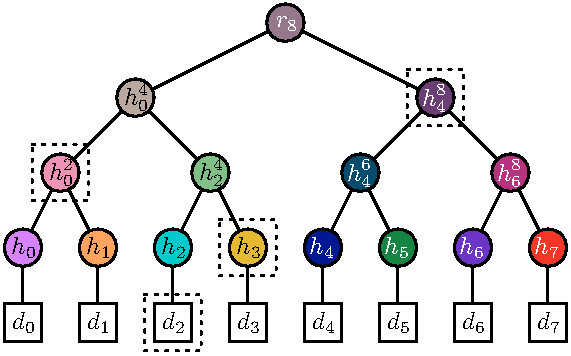
\includegraphics[width=\linewidth]{fig/mht-audit}
  \caption{Sample Merkle hash tree with eight leaf nodes. Dashed boxes indicate
  the nodes sent to prove the presence of the leaf $d_2$ in the tree.}
  \label{fig:mht-audit}
\end{figure}

A \emph{Merkle hash tree} is a binary tree in which each leaf node's value
represents data and each non-leaf node's value is the hash of its children's
values~\cite{merkle1988digital}. As shown in \autoref{fig:mht-audit}, the
structure of a Merkle hash tree allows one to efficiently prove that a data item
is present in the tree. Specifically, given the value of the root node of the
tree, one can verify the presence of any leaf node in the tree by computing a
number of hashes that is logarithmic in the number of data items in the tree.

A Merkle hash tree can store any number of nodes, i.e., the tree does not need
to be balanced. While several ways of computing the hashes in a non-balanced
tree exist, in this paper we use the method used in \ac{ct}~\cite{rfc6962}.
Specifically, given $n$ items in the Merkle hash tree, let \hashfunc be a hash
function, $d_i$ the $i$th data item (indexed from 0), and $a$ and $b$ integers
such that $0 < a < b \le n$. Then the hash of a non-leaf node representing the
$a$th to the $(b-1)$th data items is defined as
\begin{equation}
  \nodehash_a^b =
  \begin{cases}
    \hashfunc(0 \| d_a) & \mathrm{if\ } b = a + 1 \\
    \hashfunc(1 \| \nodehash_a^k \| \nodehash_k^b) & \mathrm{otherwise}
  \end{cases}
\end{equation}
where $\|$ denotes concatenation and $k = a + 2^{\lceil \log_2(b-a) \rceil - 1}$
(the largest power of 2 strictly less than $b - a$). For convenience, if $b = a
+ 1$ we write the hash as $\nodehash_a$ and call this a \emph{leaf hash}, and if
$a = 0$ and $b = n$ then we write the hash as $r_n$ and call this the \emph{root
hash}.

\begin{figure}
  \centering
  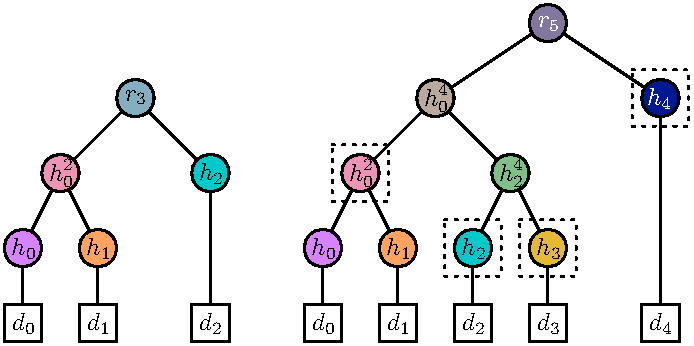
\includegraphics[width=\linewidth]{fig/mht-consistency}
  \caption{Sample Merkle hash trees with three and five data items,
  respectively. Dashed boxes indicate the nodes sent to prove consistency
between the root hashes $r_3$ and $r_5$.}
  \label{fig:mht-consistency}
\end{figure}

A Merkle hash tree can be used to implement an append-only, tamper-proof
log~\cite{crosby2009efficient}. As stated above, a Merkle hash tree can provide
an efficient \emph{proof of presence} for a given data item in the tree, thus
proving that an item was logged. To prove that the log is append-only, that is,
that no items have been changed or removed from the log, we can also use a
Merkle hash tree to provide an efficient \emph{proof of consistency} that is
logarithmic in the current size of the tree. As shown in
\autoref{fig:mht-consistency}, a proof of consistency allows one to compute the
root hash at two different times, thus showing that nodes have only been added
to the tree. A tamper-proof log would periodically sign and broadcast its root
hash, allowing clients to verify that it is not tampering with previously logged
data.

\subsection{Certificate Transparency}
\label{sec:background:ct}

\begin{figure}
  \centering
  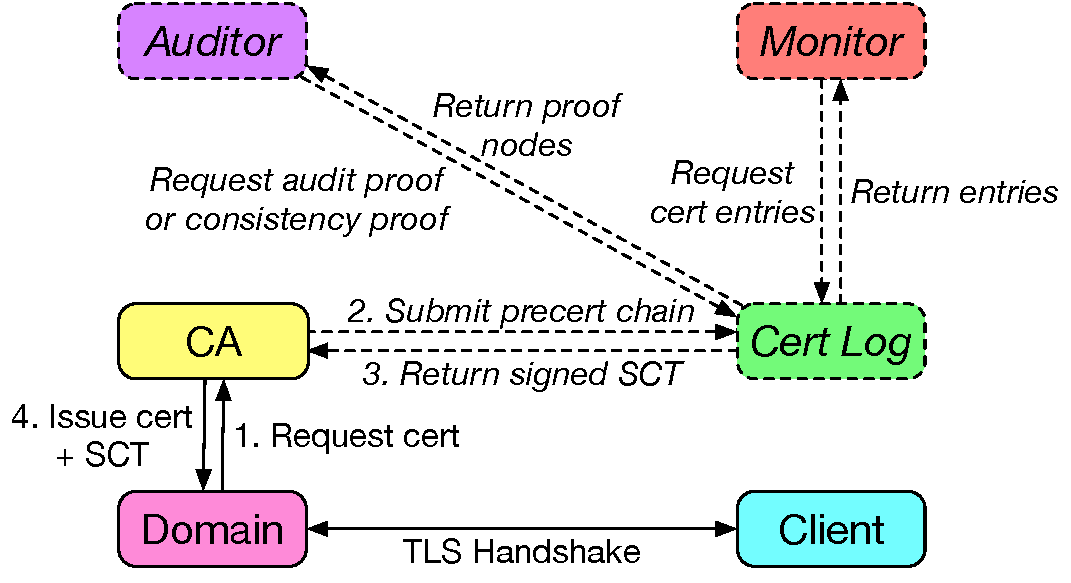
\includegraphics[width=\linewidth]{fig/ct}
  \caption{One possible configuration of the \ac{ct} architecture. Numbered
  steps denote the certificate issuance process. Dashed lines and boxes denote
entities or functions introduced by \ac{ct}, with their descriptions in
italics.}
  \label{fig:ct}
\end{figure}

\acf{ct} is a project by Google focused on enabling widespread detection of
certificate issuance~\cite{rfc6962}. As shown in \autoref{fig:ct}, \ac{ct}
introduces several new roles to the \ac{ca}-based ecosystem. \emph{Certificate
logs} are entities who record \ac{ca} behavior by maintaining a publicly
auditable, append-only, tamper-proof database of certificates. \emph{Monitors}
periodically retrieve these certificates to check for suspicious \ac{ca}
behavior, such as an obscure \ac{ca} issuing a certificate for Google.
\emph{Auditors} check for correct log behavior by periodically asking for
\emph{audit proofs}, which show that one or more certificates are in a log
database, or \emph{consistency proofs}, which show that the existing database
has not been tampered with, i.e., that no certificate has been changed, deleted,
or retroactively added to the log database.

A log leverages Merkle hash trees to implement its certificate database. As
explained above, the use of a Merkle hash tree allows a log to provide efficient
proofs of presence (i.e., audit proofs) and proofs of consistency (i.e.,
consistency proofs). While anyone may submit a certificate to a log, in current
practice \acp{ca} usually log certificates during the issuance process, as
depicted in \autoref{fig:ct}. Because attempting to update the Merkle hash tree
in real time may delay or block the certificate issuance process, logs define a
\emph{\ac{mmd}}, a time period after which a certificate is guaranteed to be
logged, and instead return a \emph{\ac{sct}}, which is effectively a promise to
add the certificate within the \ac{mmd}. The \ac{sct} is embedded into the
\ac{ca}-issued certificate as an X.509 extension and used to signal that a
domain uses \ac{ct} and that its certificate has been logged. Alternately, the
domain can send extra information such as \acp{sct} or audit proofs in the
\ac{tls} handshake using a \ac{tls} protocol extension.

\draft{Monitoring and auditing details. Monitors periodically downloads all new
  entries and verifies consistency proof. Does not need to keep cert entries
  after finishing. Auditors periodically query for random audit proofs or
  consistency proofs. Specifically, can pass a cert hash and a size of the tree
  and get an audit proof in return, or pass two sizes of the tree and get a
  consistency proof in return. To verify this information, log also provides a
  function to get the latest signed tree head. In order to detect
  \emph{equivocation} (i.e., showing different versions of the log to different
  queries), auditors must gossip tree heads. The log's public key is known
  through a trusted entity such as Google.}

\draft{\ac{ct} does not check for revocation, though multiple extensions
designed to handle revocation have been proposed (see \autoref{sec:related}).
Perhaps the easiest way to do to this is to create a new Merkle hash tree every
\ac{mmd} that contains as its leaves the list of \emph{currently valid}
certificates.}
